%=======================+=========================
%================  Online  ================
%=================================================

%------------------------------------------------------------------
\section[Online computing system (David)]{Online computing system \label{sec:online}}
\subsection{Monitoring \label{sec:onlinemonitoring}}

The Online Monitoring system (OMS) consists of several parts that provide for immediate monitoring of the data, as well near term monitoring ($\sim$hours after acquisition). The immediate monitoring is based on the \textit{RootSpy}\cite{rootspy} system. Figure \ref{fig:online_monitoring_processes} shows a diagram of the processes involved in the RootSpy system and how they couple to the DAQ system using the Event Transfer (ET) software package. ET is part of the CODA DAQ system\cite{coda} and can be used to extract a copy of the data without interfering with the DAQ. The monitoring system utilizes a secondary ET in order to minimize connections to the RAID server running the ER ensuring minimal potential impact to the DAQ.

\begin{figure}[tbp]
\begin{center}
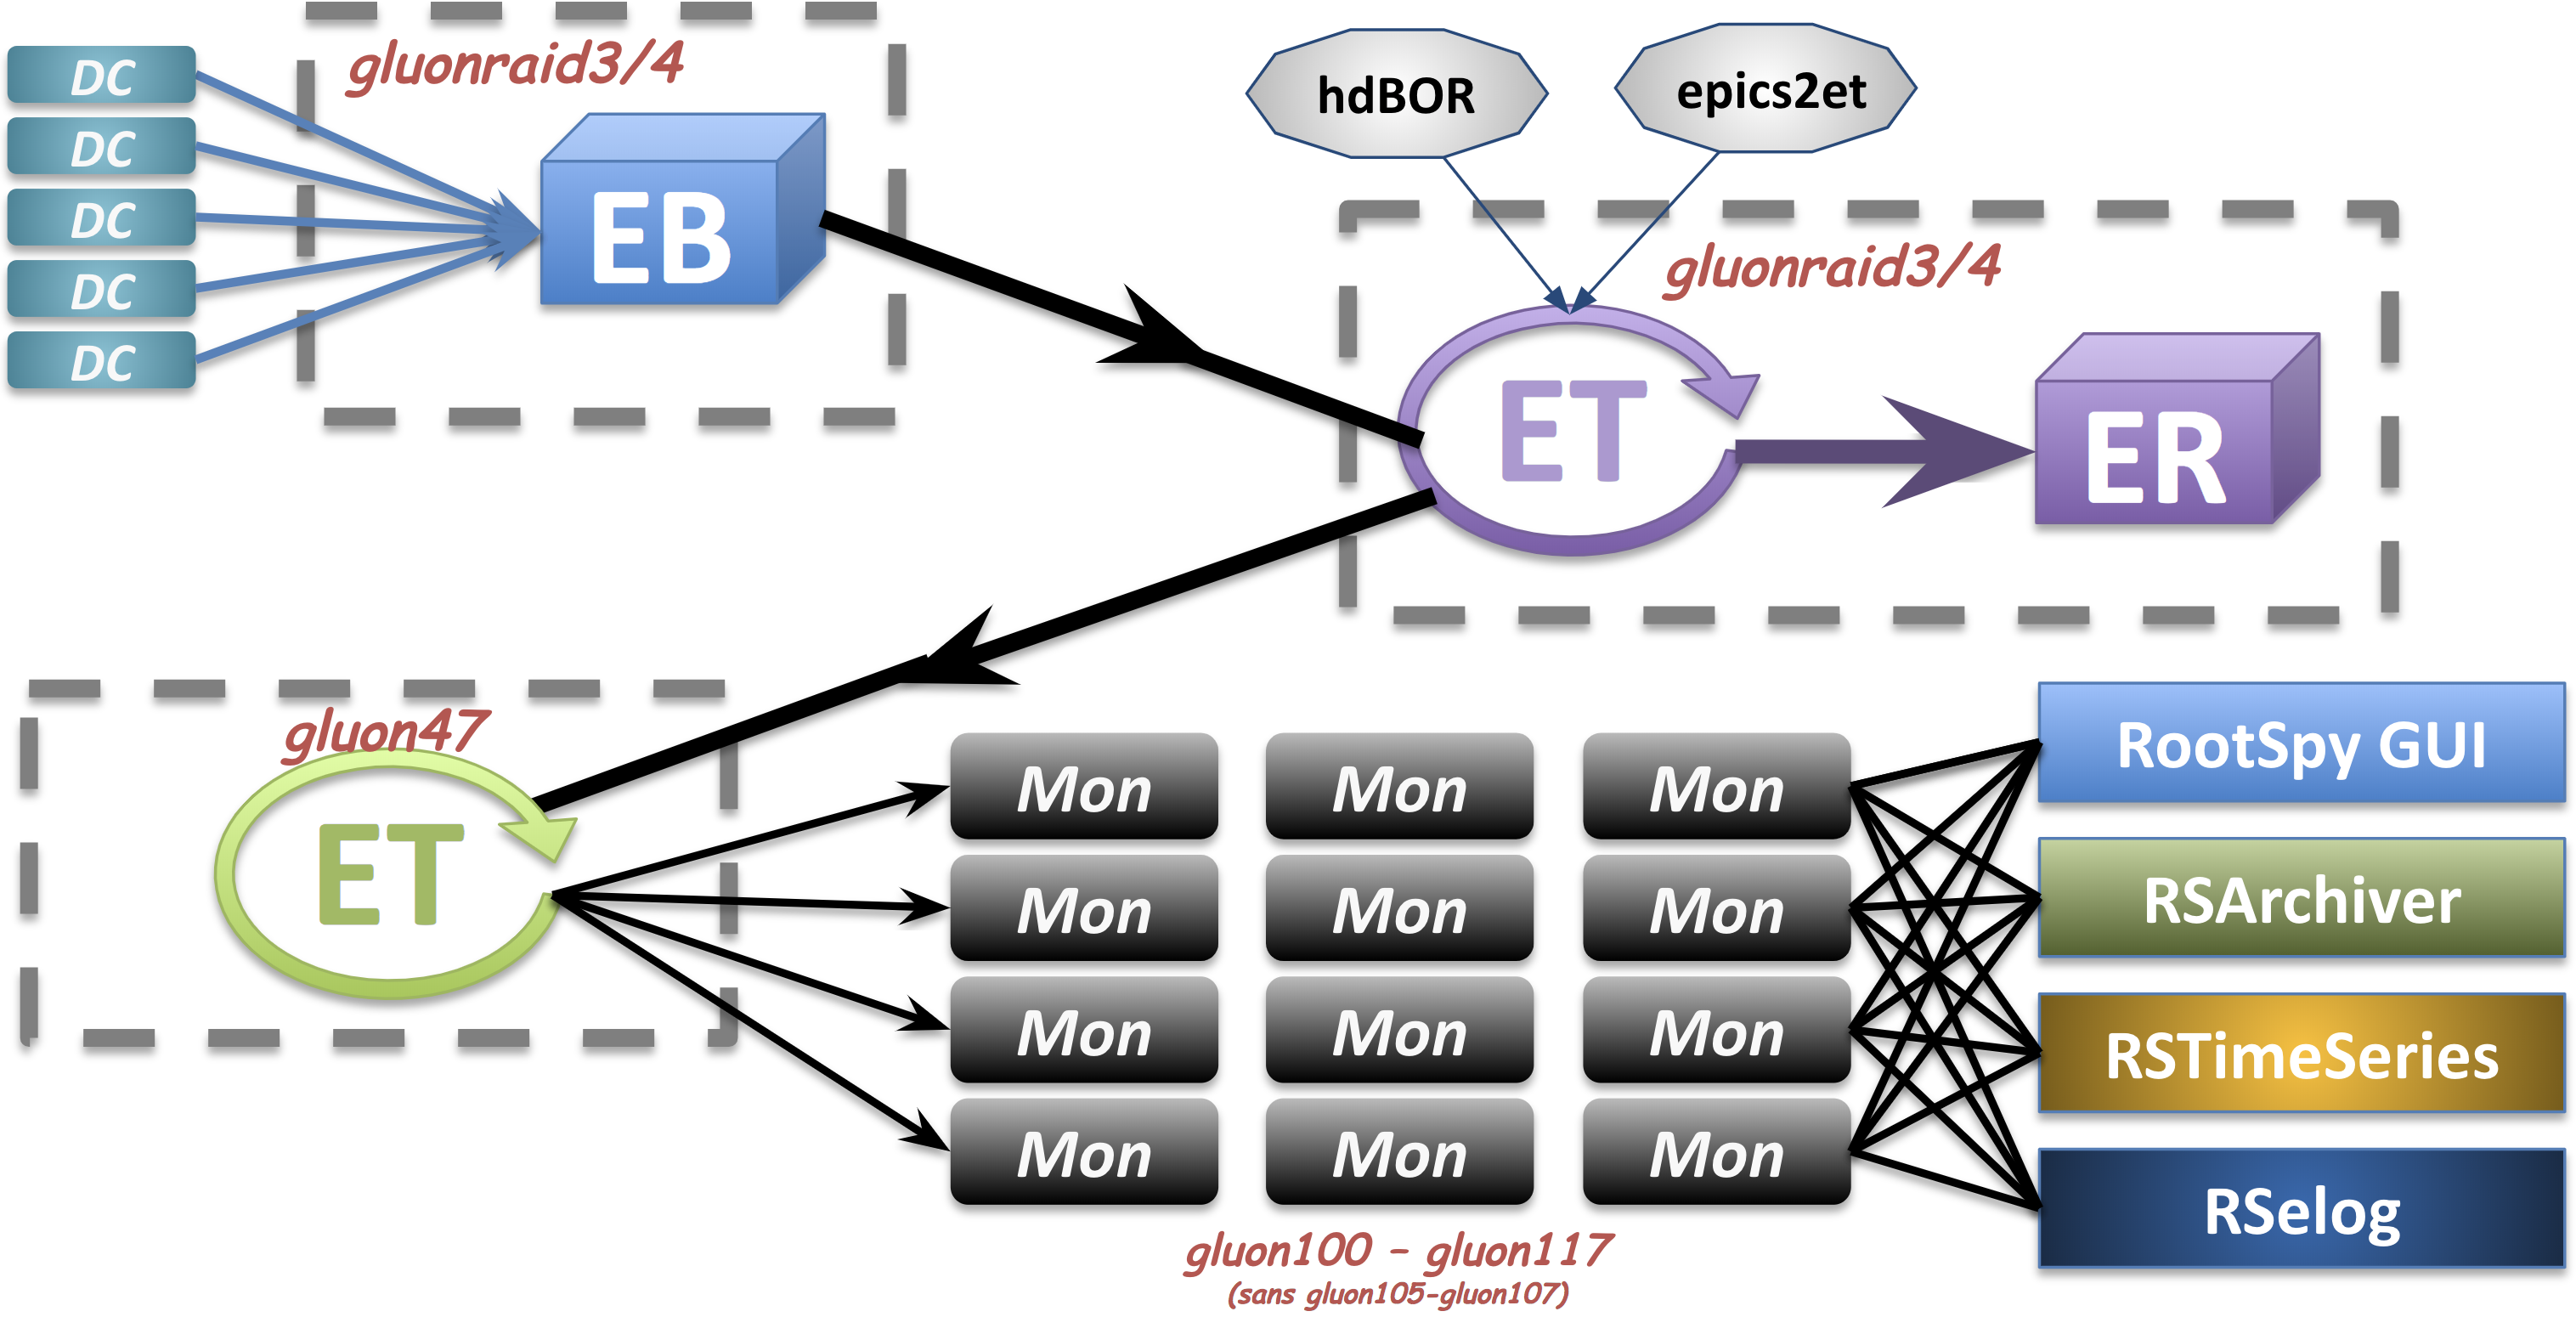
\includegraphics[width=0.99\textwidth]{figures/online_monitoring_processes.png}
\label{fig:online_monitoring_processes}
\caption{Diagram of the various processes distributed across several computers in the counting house that make up the online monitoring system. DC, EB, and ER represent the Data Concentrator, Event Builder, and Event Recorder processes respectively in the CODA DAQ system.}   
\end{center}  
\end{figure}

RootSpy was developed at JLab for GlueX, though its design is not GlueX specific. The system is run on a small farm of 12 computers in the counting house, each processing a small part of the data stream. ET is used to distribute the data among the farm computers. Each farm node generates histogram which RootSpy gathers and combines before displaying to shift workers in a GUI. Figure \ref{fig:online_monitoring_rootspy} shows a screen capture of the main RootSpy GUI window along with a window displaying the reference plot for the currently displayed image. The main RootSpy window allows plots to be grouped into tabs and for users to step through the plots either via mouse click or automatically. Shift workers may use the GUI to set any plot as the new reference for that plot. An e-mail is automatically sent when this is done to a list of addresses associated with the plot. The e-mail includes the old and new reference images so that system experts receiving the e-mail can see when a new reference is installed and how it differs from the previous.

\begin{figure}[tbp]
\begin{center}
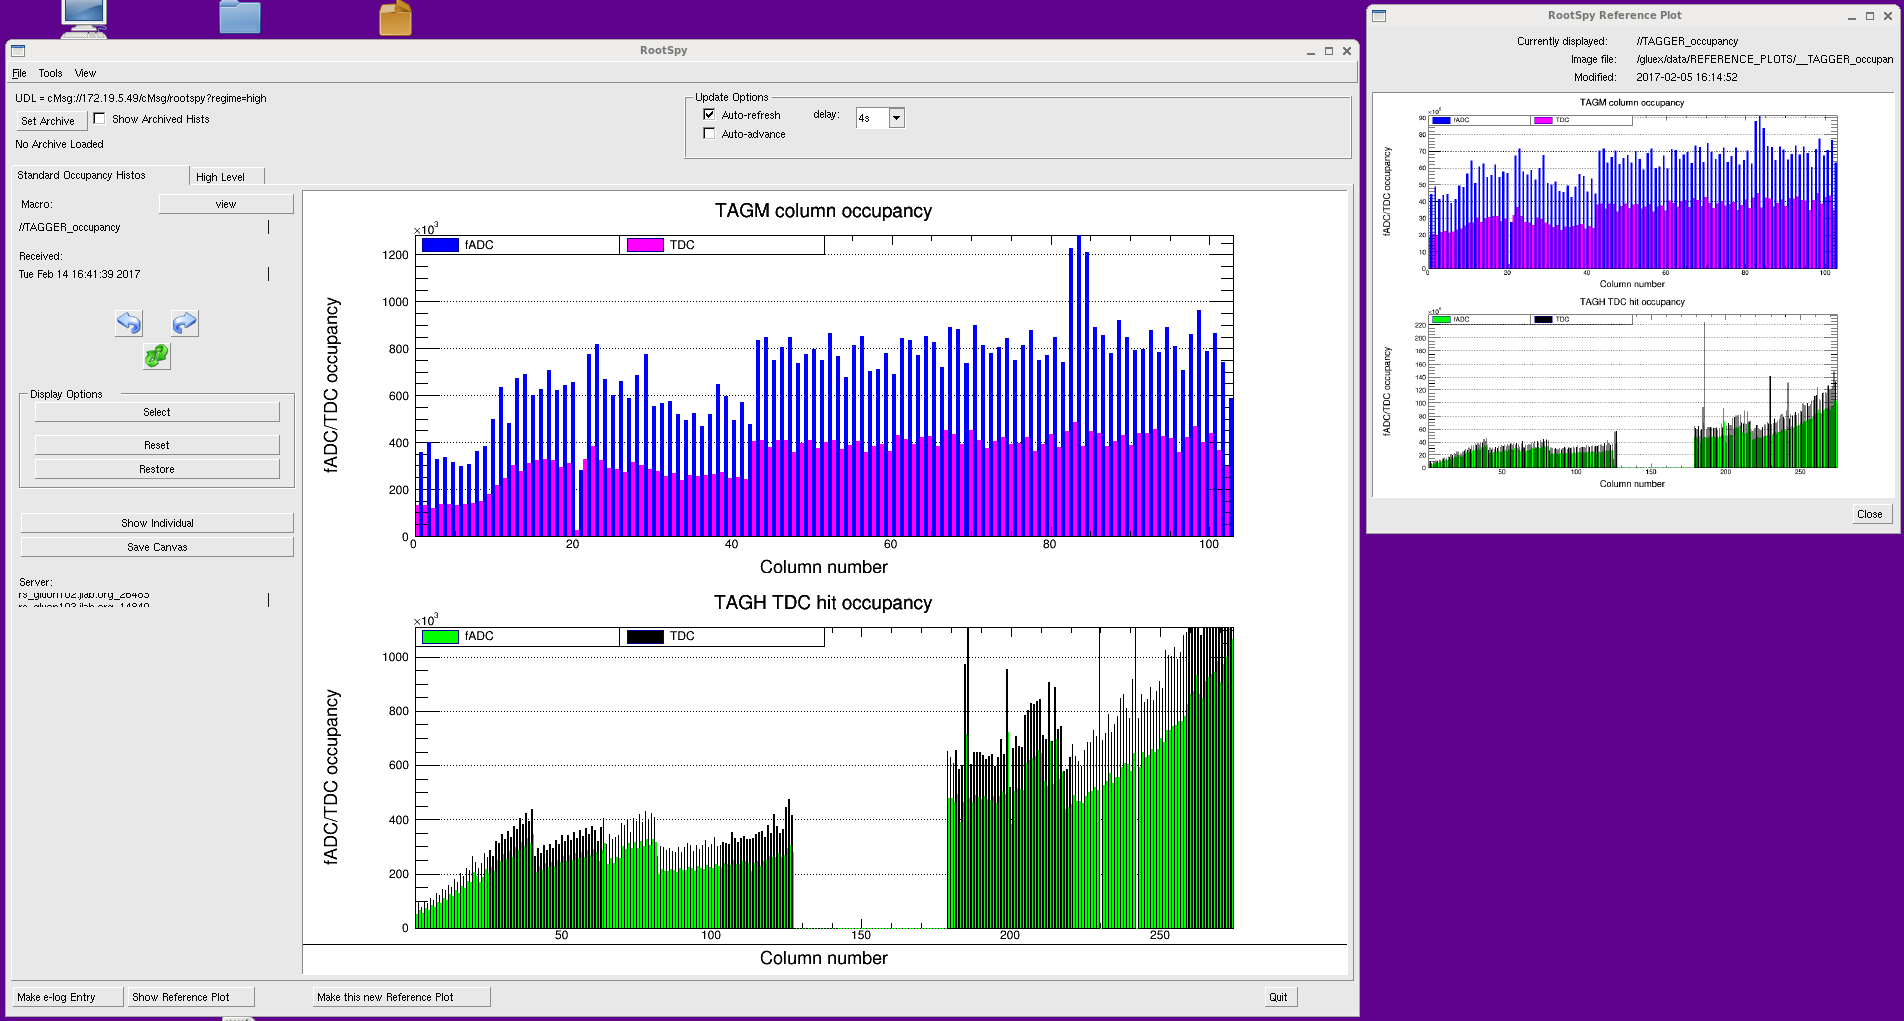
\includegraphics[width=0.99\textwidth]{figures/online_monitoring_rootspy.png}
\label{fig:online_monitoring_rootspy}
\caption{Screen capture of the RootSpy GUI program main window and the reference image in the upper right.}   
\end{center}  
\end{figure}

Each farm node runs a JANA\cite{jana} process that links the same GlueX libraries used in the final reconstruction of GlueX data. Three of the monitoring computers are dedicated to ``occupancy'' plots which allows them to process events at a much higher rate since they do not perform full event reconstruction. The remaining eight monitoring computers produce these same plots and in addition do perform full event reconstruction. 
Figure \ref{fig:online_monitoring_PID} shows an example of a plot made using full event reconstruction. Figure \ref{fig:online_monitoring_digihits} shows an example of an occupancy level plot. In this plot the number of hit objects per event are shown for various detector hit types. The mean values for each hit type are shown in the grey boxes at the top while scale factors used for display are shown in grey boxes along the middle. 
\begin{figure}[tbp]
\begin{center}
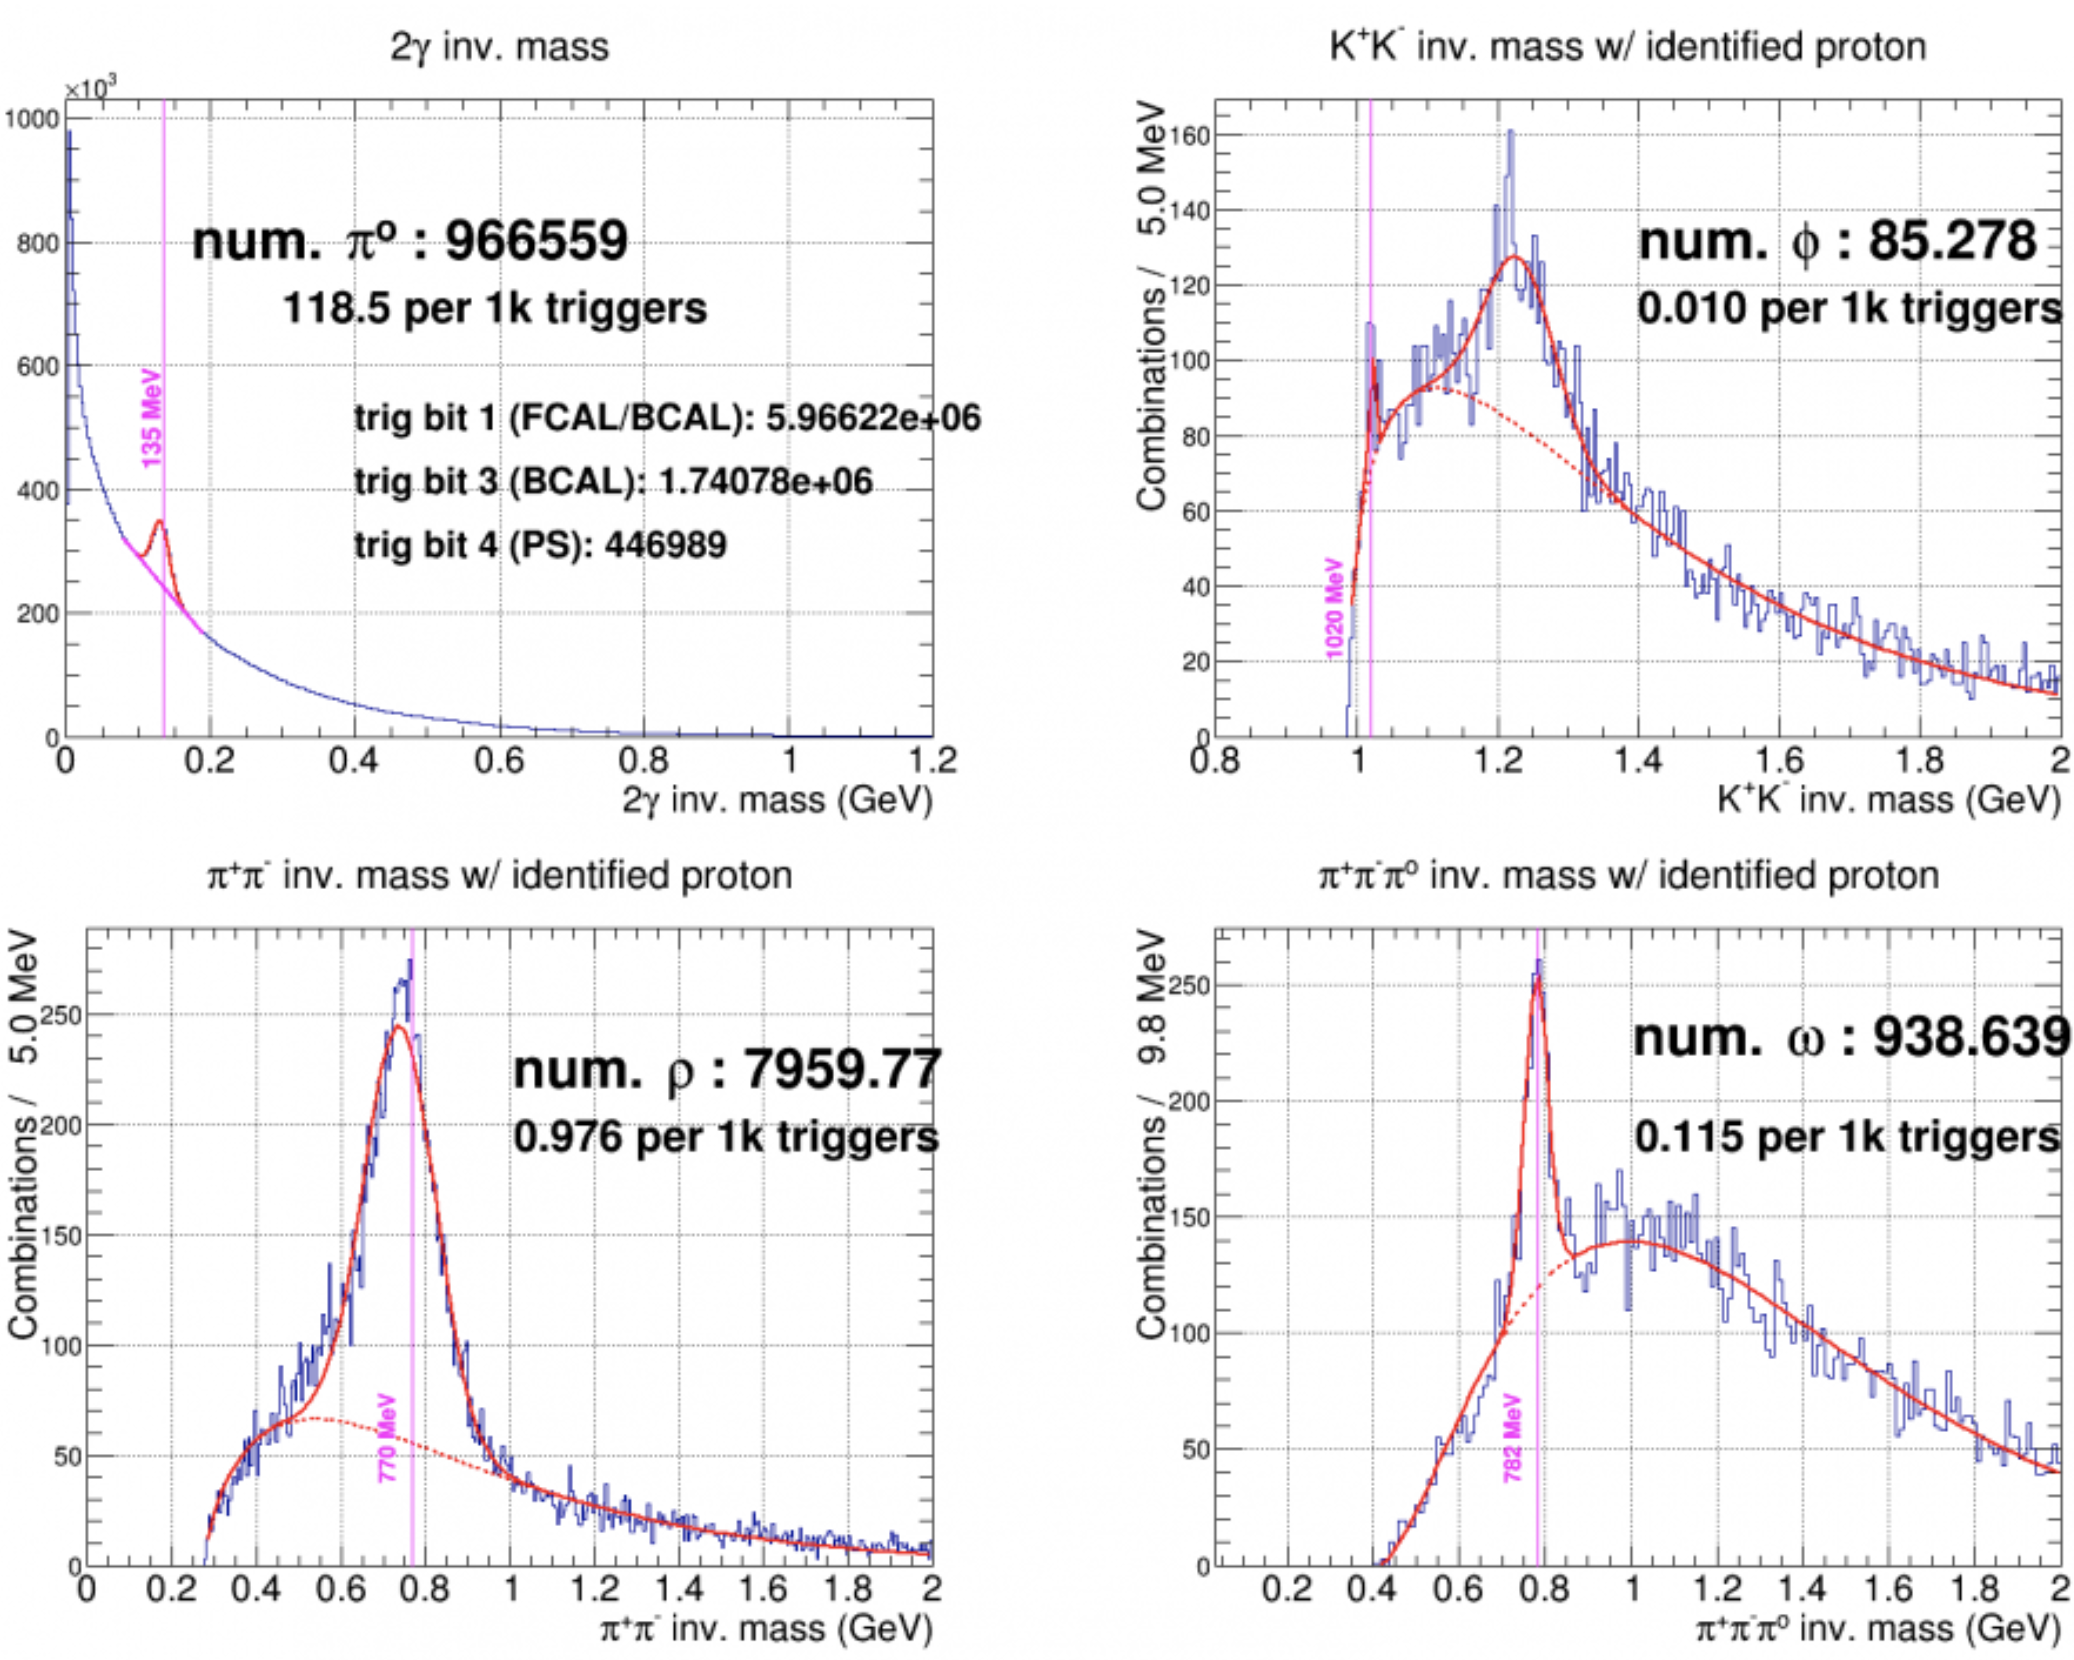
\includegraphics[width=0.99\textwidth]{figures/online_monitoring_PID.png}
\label{fig:online_monitoring_PID}
\caption{Invariant mass distributions showing $\pi^\circ$, $\omega$, $\rho$, and $\phi$ particles.}   
\end{center}  
\end{figure}

\begin{figure}[tbp]
\begin{center}
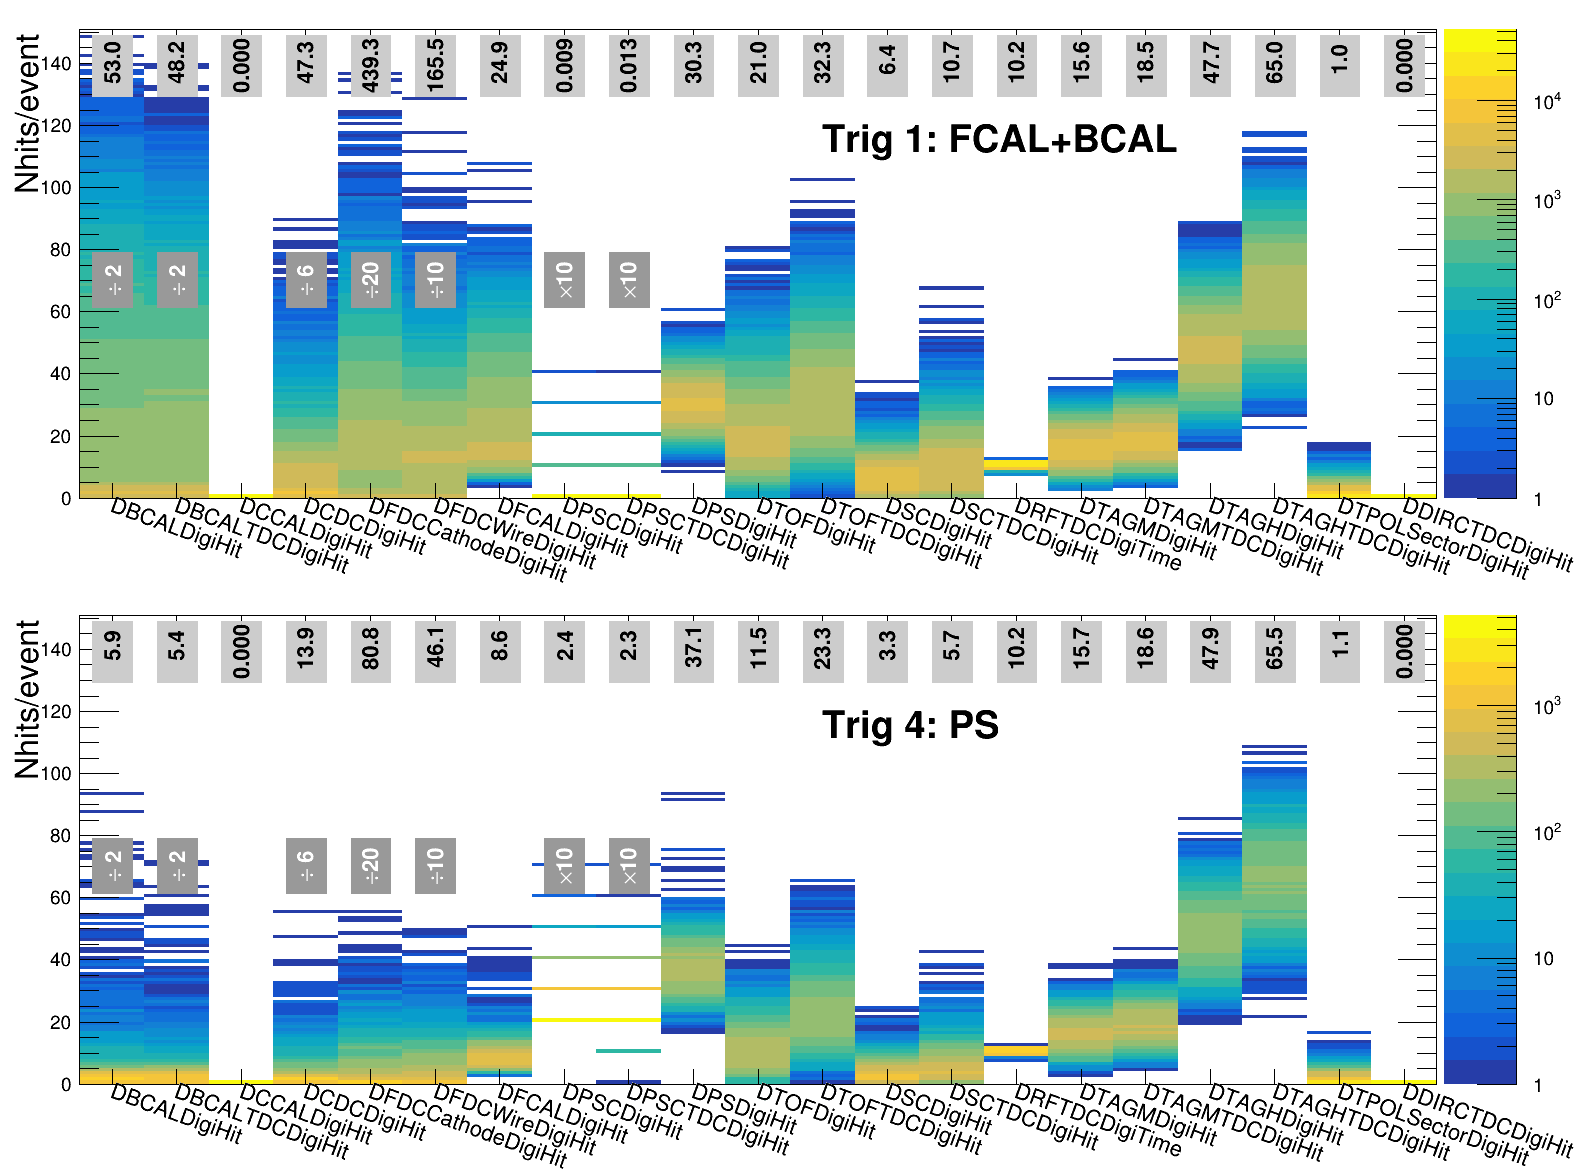
\includegraphics[width=0.99\textwidth]{figures/online_monitoring_digihits.png}
\label{fig:online_monitoring_digihits}
\caption{Example monitoring plot showing the number of low-level hit objects per event separated by trigger type. Some have the y-values are scaled by factors shown in the grey boxes so that they comfortably fit on the same plot.}   
\end{center}  
\end{figure}

Plots are drawn in RootSpy via ROOT macros that are transported using the same xMsg\cite{xmsg} publish subscribe messaging system used to transport histogram objects. The macros are compiled into plugins as C++ strings by the build system. The build system recognizes ROOT macro files in the plugin source directory (via the .C suffix) and automatically generates C++ code that contains the macro and code to register it with the RootSpy system. This is done to ensure that the macro is always in sync with the histograms being produced by a given plugin since the macros and histograms are always sent from the same binary. This also enforces keeping the plugin and macro source in the same repository directory making it easier for multiple people to maintain the code.

In addition to the RootSpy GUI, several other client programs exist that consume the histograms being produced by the farm nodes. One of these is the RSTimeSeries program. This program runs in the background periodically running macros that contain special calls to insert data into an InfluxDB time series database. These are the same macros used to produce the plots shift workers view with the RootSpy GUI. The macros have special calls enabling to send entries to the InfluxDB whenever a statistics threshold is met for a given quantity. Examples of these are shown in figures \ref{fig:online_monitoring_grafana1} and \ref{fig:online_monitoring_grafana2}. Figure \ref{fig:online_monitoring_grafana2} shows a strip chart of the particles per 1k triggers extracted from the same macro used to draw figure \ref{fig:online_monitoring_PID}.

\begin{figure}[tbp]
\begin{center}
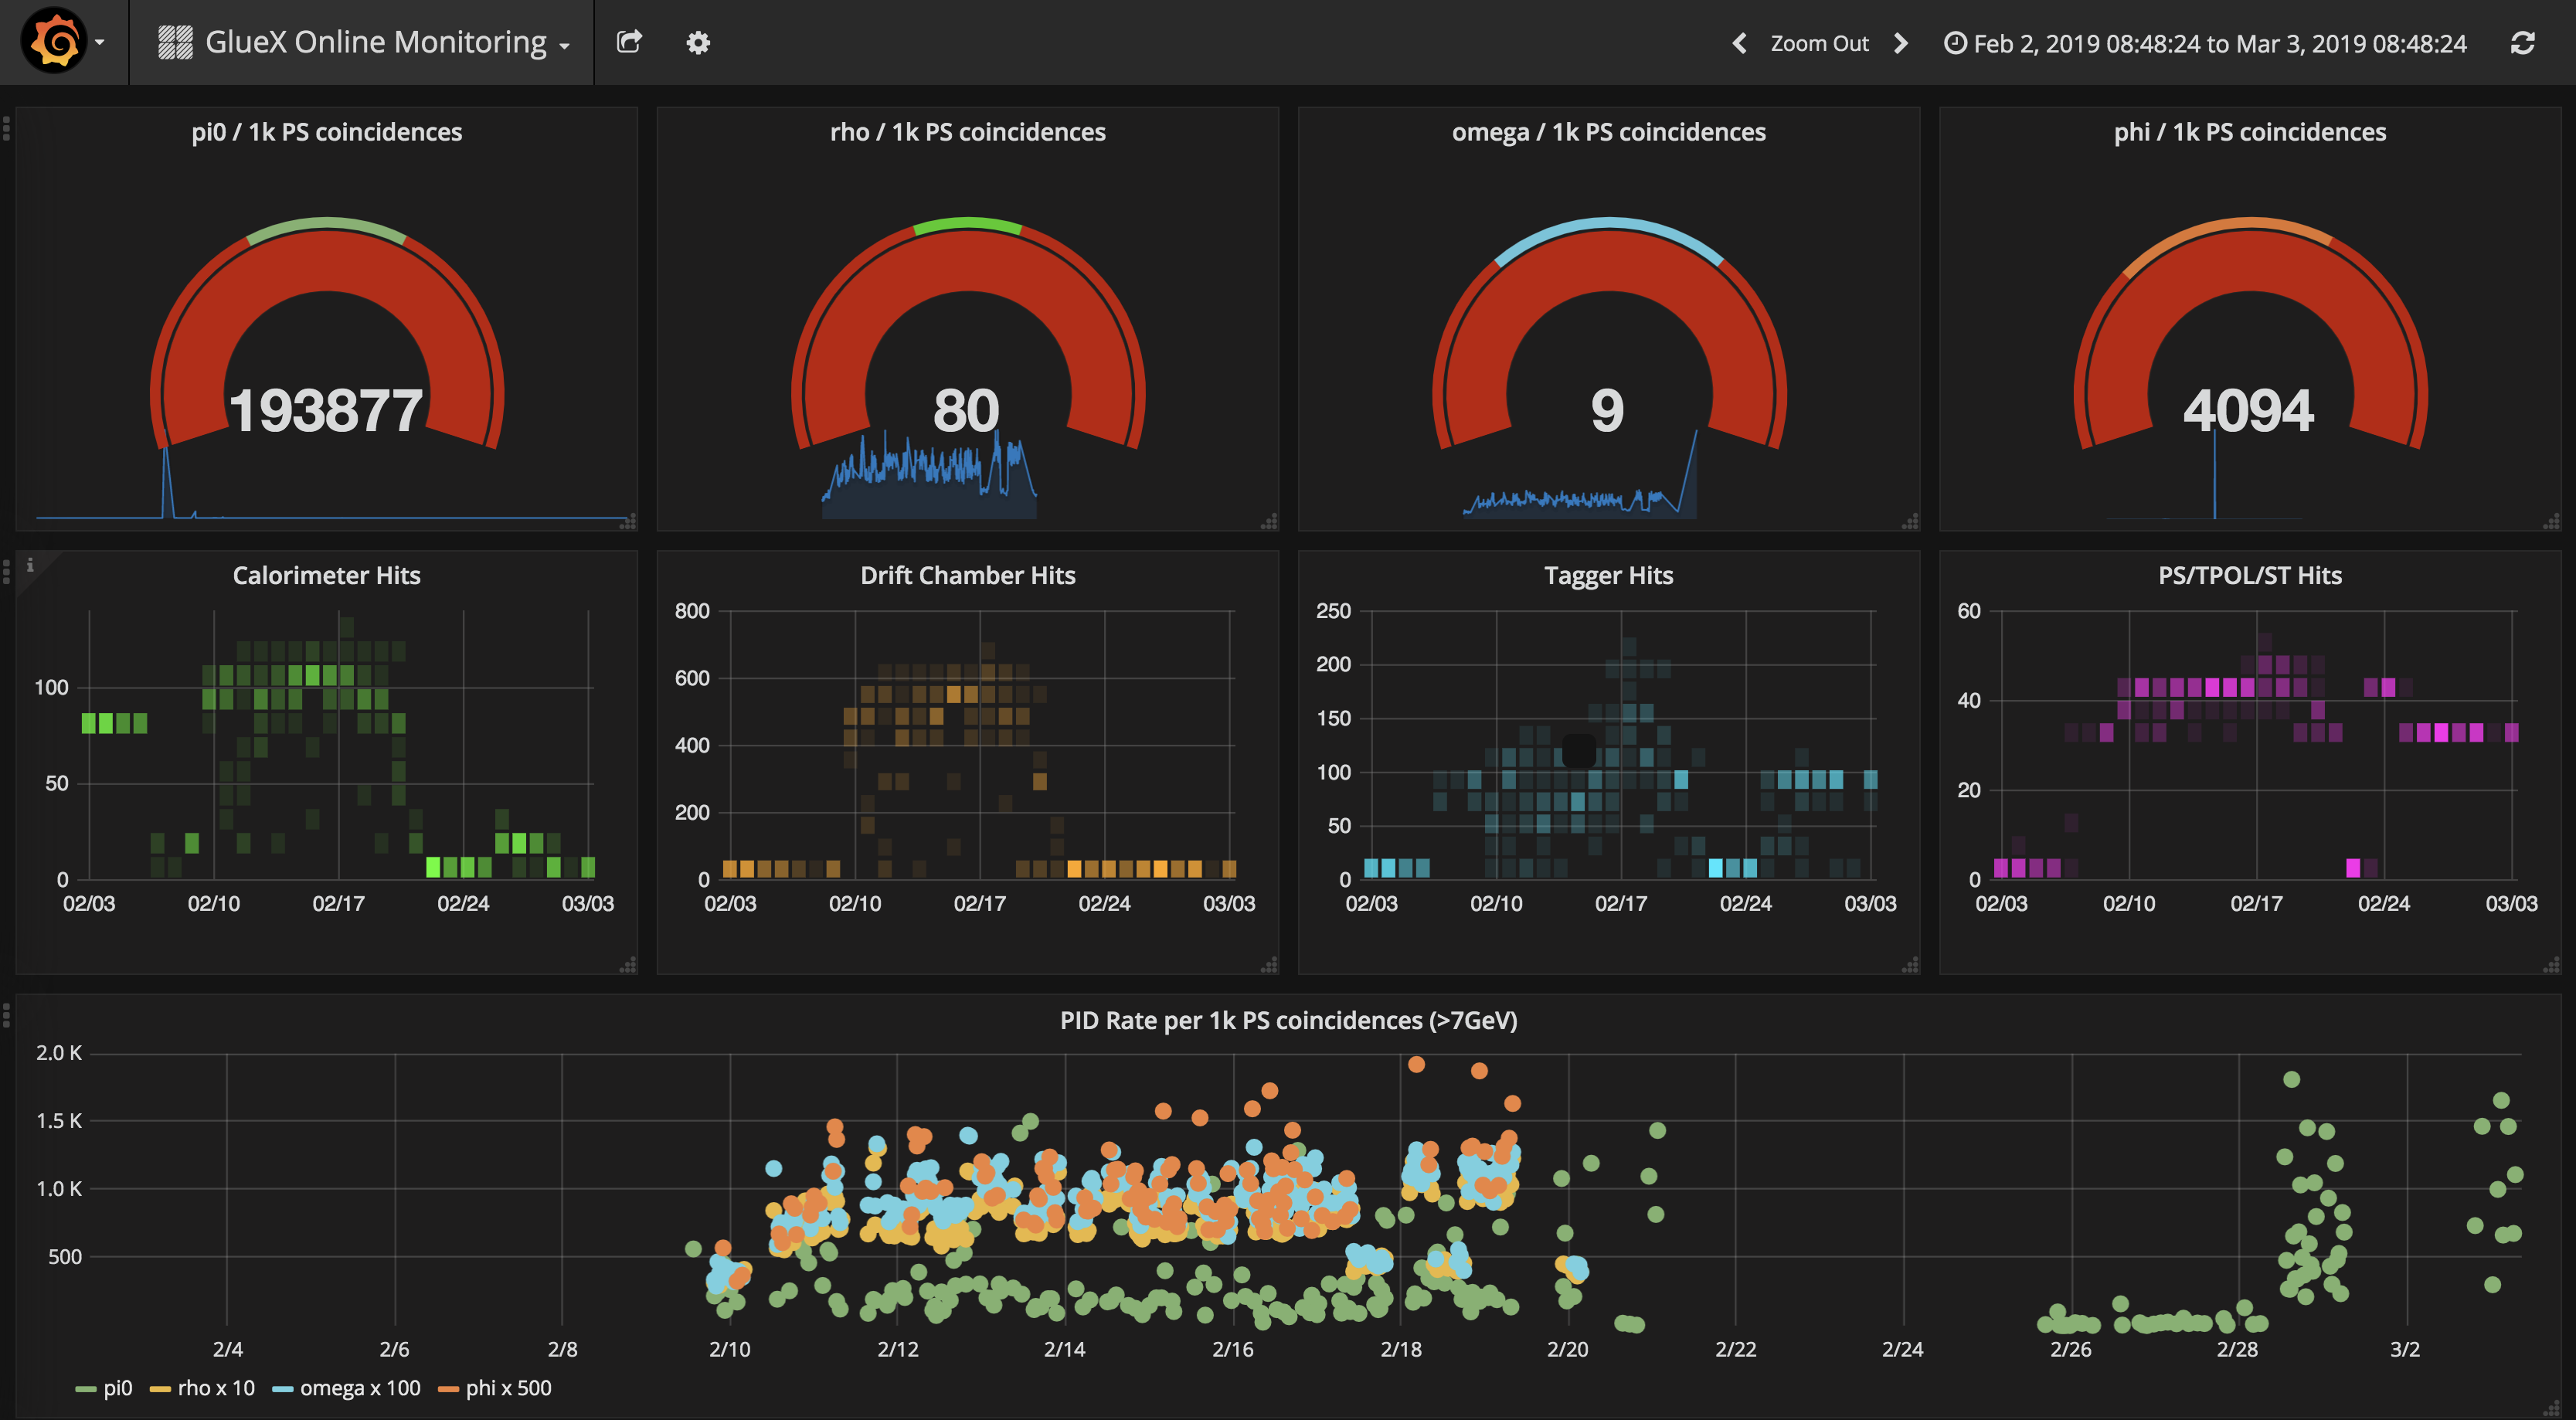
\includegraphics[width=0.99\textwidth]{figures/online_monitoring_grafana1.png}
\label{fig:online_monitoring_grafana1}
\caption{Screen capture of Grafana driven web site showing reconstructed particle rates and detector hit rates as a function of time.}
\end{center}  
\end{figure}

\begin{figure}[tbp]
\begin{center}
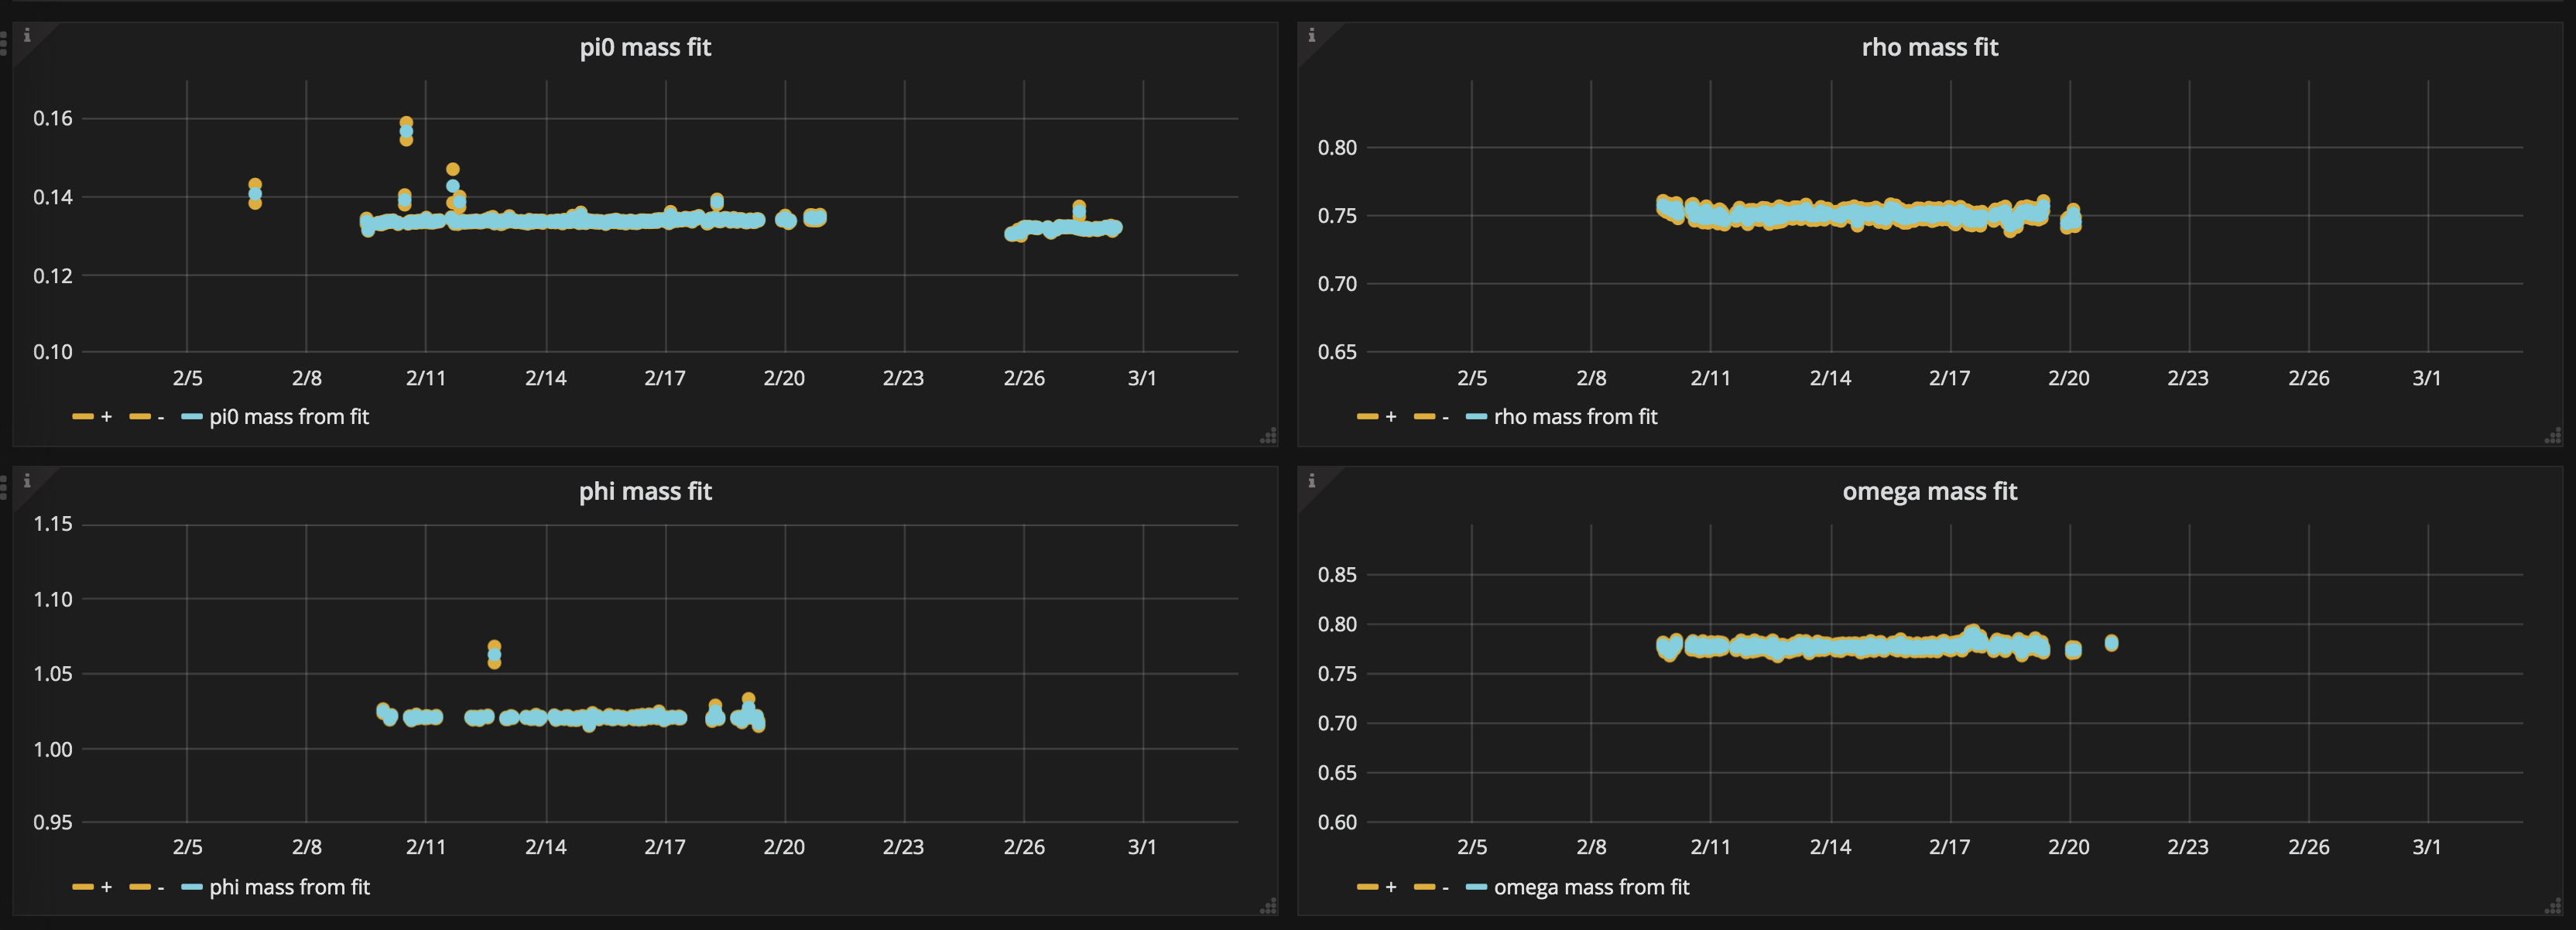
\includegraphics[width=0.99\textwidth]{figures/online_monitoring_grafana2.png}
\label{fig:online_monitoring_grafana2}
\caption{Online strip charts of particle rates per trigger. The online monitoring system does full reconstruction of 2\%-3\% of events as the data is acquired.}   
\end{center}  
\end{figure}

\begin{figure}[tbp]
\begin{center}
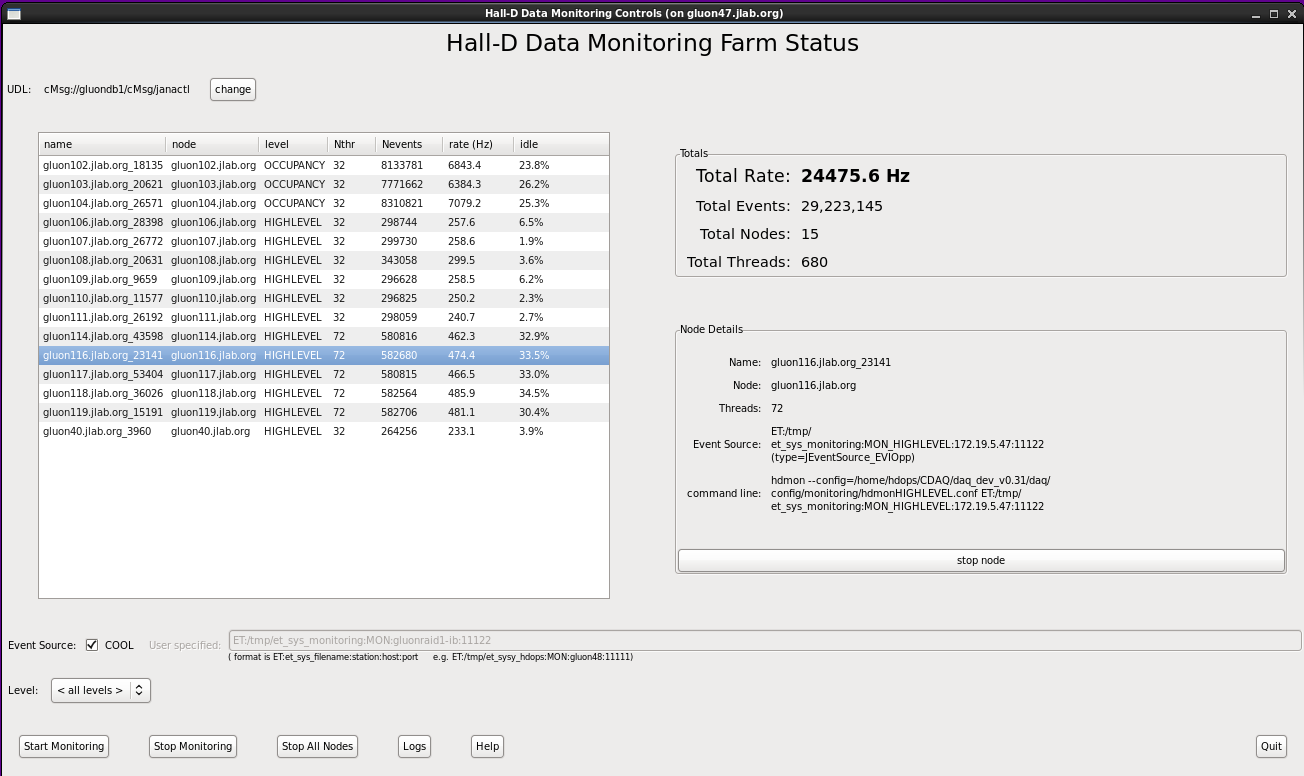
\includegraphics[width=0.99\textwidth]{figures/online_monitoring_hdmongui.png}
\label{fig:online_monitoring_hdmongui}
\caption{GUI interface to online monitoring system.}   
\end{center}  
\end{figure}

PLOT BROWSER


%------------------------------------------------------------------
\subsection{Online event processing \label{sec:onlineprocessing}}

\begin{figure}[tbp]
\begin{center}
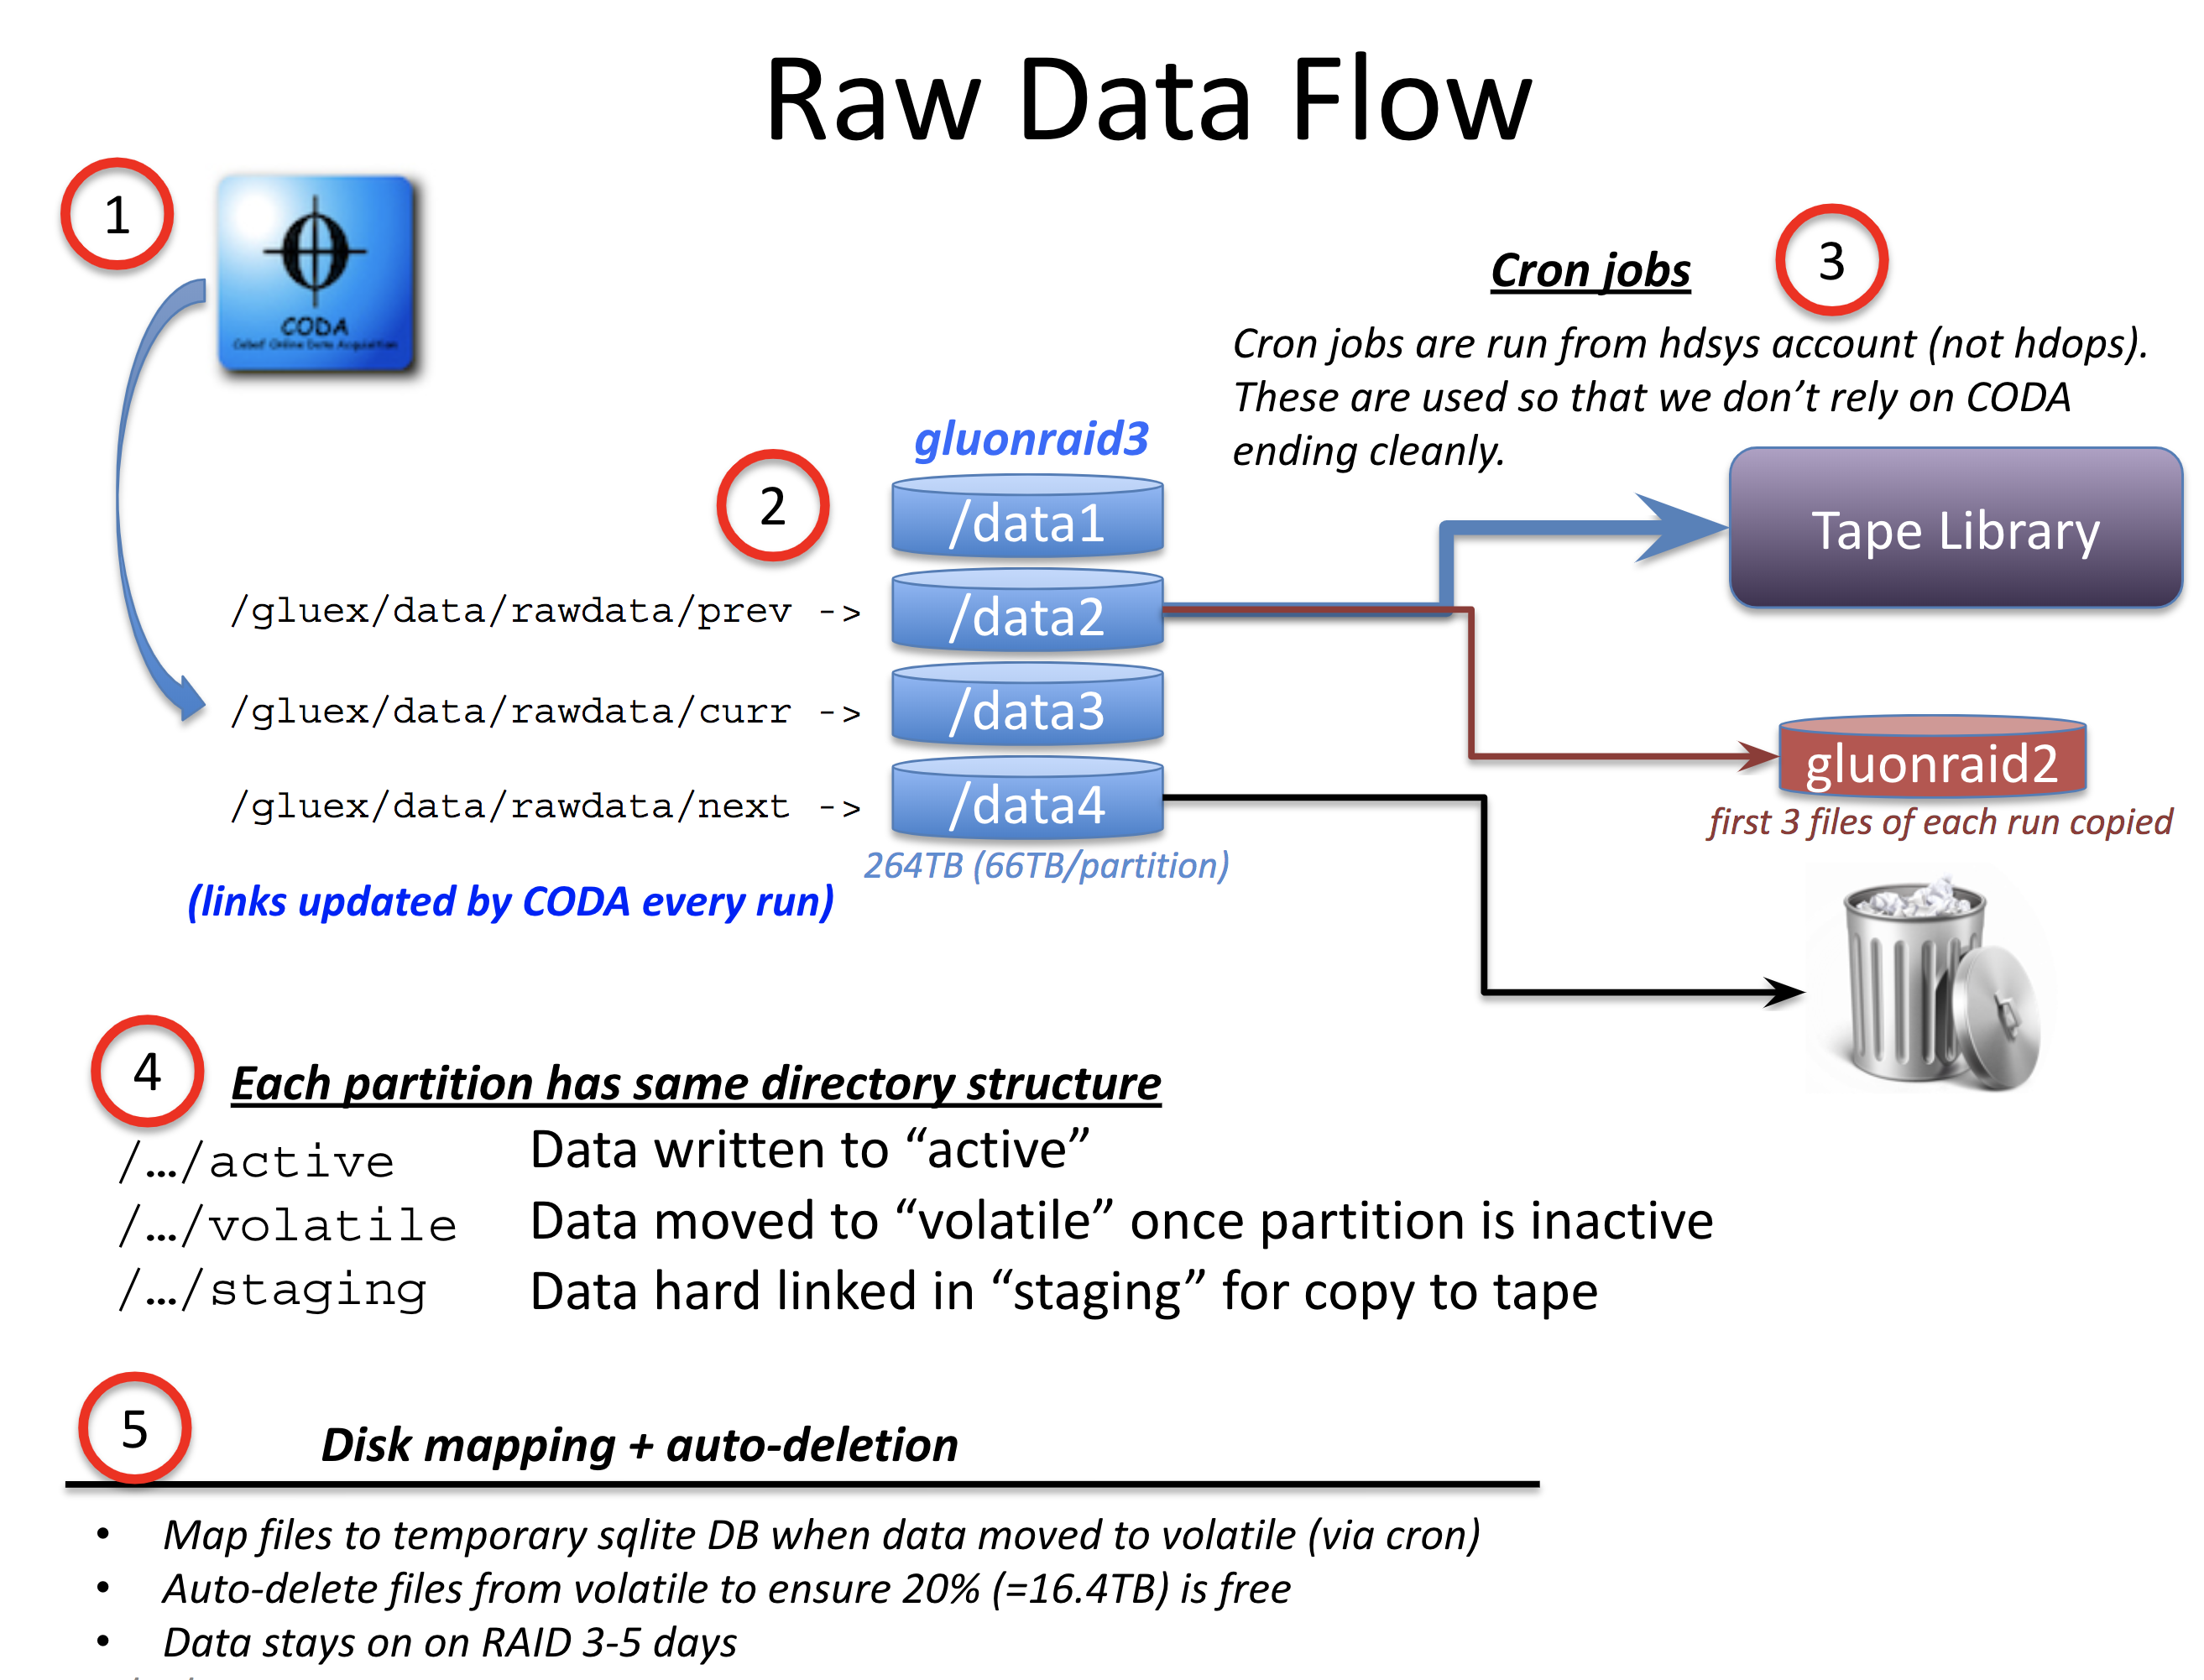
\includegraphics[width=0.99\textwidth]{figures/online_dataflow.png}
\label{fig:online_dataflow}
\caption{Diagram of the data transport system used to move the data through the temporary RAID storage system to tape.}   
\end{center}  
\end{figure}
